\documentclass{beamer}
\mode<presentation>
\usepackage{amsmath}
\usepackage{amssymb}
%\usepackage{advdate}
\usepackage{adjustbox}
\usepackage{subcaption}
\usepackage{enumitem}
\usepackage{multicol}
\usepackage{mathtools}
\usepackage{listings}
\usepackage{url}
\def\UrlBreaks{\do\/\do-}
\usetheme{Boadilla}
\usecolortheme{lily}
\setbeamertemplate{footline}
{
  \leavevmode%
  \hbox{%
  \begin{beamercolorbox}[wd=\paperwidth,ht=2.25ex,dp=1ex,right]{author in head/foot}%
    \insertframenumber{} / \inserttotalframenumber\hspace*{2ex} 
  \end{beamercolorbox}}%
  \vskip0pt%
}
\setbeamertemplate{navigation symbols}{}

\providecommand{\nCr}[2]{\,^{#1}C_{#2}} % nCr
\providecommand{\nPr}[2]{\,^{#1}P_{#2}} % nPr
\providecommand{\mbf}{\mathbf}
\providecommand{\pr}[1]{\ensuremath{\Pr\left(#1\right)}}
\providecommand{\qfunc}[1]{\ensuremath{Q\left(#1\right)}}
\providecommand{\sbrak}[1]{\ensuremath{{}\left[#1\right]}}
\providecommand{\lsbrak}[1]{\ensuremath{{}\left[#1\right.}}
\providecommand{\rsbrak}[1]{\ensuremath{{}\left.#1\right]}}
\providecommand{\brak}[1]{\ensuremath{\left(#1\right)}}
\providecommand{\lbrak}[1]{\ensuremath{\left(#1\right.}}
\providecommand{\rbrak}[1]{\ensuremath{\left.#1\right)}}
\providecommand{\cbrak}[1]{\ensuremath{\left\{#1\right\}}}
\providecommand{\lcbrak}[1]{\ensuremath{\left\{#1\right.}}
\providecommand{\rcbrak}[1]{\ensuremath{\left.#1\right\}}}
\theoremstyle{remark}
\newtheorem{rem}{Remark}
\newcommand{\sgn}{\mathop{\mathrm{sgn}}}
\providecommand{\abs}[1]{\left\vert#1\right\vert}
\providecommand{\res}[1]{\Res\displaylimits_{#1}} 
\providecommand{\norm}[1]{\lVert#1\rVert}
\providecommand{\mtx}[1]{\mathbf{#1}}
\providecommand{\mean}[1]{E\left[ #1 \right]}
\providecommand{\fourier}{\overset{\mathcal{F}}{ \rightleftharpoons}}
%\providecommand{\hilbert}{\overset{\mathcal{H}}{ \rightleftharpoons}}
\providecommand{\system}{\overset{\mathcal{H}}{ \longleftrightarrow}}
	%\newcommand{\solution}[2]{\textbf{Solution:}{#1}}
%\newcommand{\solution}{\noindent \textbf{Solution: }}
\providecommand{\dec}[2]{\ensuremath{\overset{#1}{\underset{#2}{\gtrless}}}}
\newcommand{\myvec}[1]{\ensuremath{\begin{pmatrix}#1\end{pmatrix}}}
\let\vec\mathbf

\lstset{
%language=C,
frame=single, 
breaklines=true,
columns=fullflexible
}

\numberwithin{equation}{section}

\title{1.6.7}
\author{Rushil Shanmukha Srinivas \\EE25BTECH11057 \\ Electrical Enggineering ,\\IIT Hyderabad.}

\date{\today} 
\begin{document} 

\begin{frame}
\titlepage
\end{frame}

\section*{Outline}
\begin{frame}
\tableofcontents
\end{frame}
\section{Problem}
\begin{frame}
\frametitle{Problem Statement}

Find a relation between x and y if the points (x,y) ,(1,2) and (7,0) are collinear.
\\ \begin{table}[h!]    
  \centering
  \begin{center}
\begin{tabular}{ll}
    \textbf{Group I} & \textbf{Group II} \\
    P. Ferrite & 1. Hexagonal Close Packed (HCP) \\
    Q. Austenite & 2. Body Centered Cubic (BCC) \\
    R. Martensite & 3. Body Centered Tetragonal (BCT) \\
    & 4. Face Centered Cubic (FCC)
\end{tabular}
\end{center}
  \caption{Variables Used}
\end{table}
\end{frame}
\section{Solution}
\subsection{Collinearity of Matrix}
\begin{frame}
\frametitle{Collinearity of Matrix}
%\framesubtitle{Literature}
Let the three points be
$
\vec{A}=\myvec {x \\ y} ,\quad
\vec{B}=\myvec {1 \\ 2} , \quad 
\vec{C}=\myvec {7 \\ 0}.
$
\\

For collinearity, 
\begin{align}
\operatorname{rank}\!\Big( \myvec {\vec{B}-\vec{A} & \vec{C}-\vec{A} }^T \Big) = 1.
\end{align}

Now,
\begin{align}
\vec{B}-\vec{A} = \myvec{1-x \\ 2-y} , \quad
\vec{C}-\vec{A} = \myvec{7-x \\ -y}.
\end{align}

So the matrix is
\begin{align}
\vec{M} = \myvec {\vec{B}-\vec{A} & \vec{C}-\vec{A} }^T
= \myvec{
1-x & 2-y \\
7-x & -y}.
\end{align}
\end{frame}
\subsection{Echelon Form and Row Operations}
\begin{frame}
\frametitle{Echelon Form and Row Operations}
\subsection*{Row Reduction}

Step 1: Start with
\begin{align}
\vec{M} = \myvec
{1-x & 2-y \\
7-x & -y}.
\end{align}

Step 2: Eliminate the first entry of the second row:

\begin{align}
R_2 \;\longrightarrow\; R_2 - \frac{7-x}{\,1-x\,}R_1 \quad (\text{assuming } x\neq 1).
\end{align}

\begin{align}
\myvec
{1-x & 2-y \\
7-x & -y}
\;\;\longrightarrow\;\;
\myvec
{1-x & 2-y \\
0 & -y - \frac{7-x}{\,1-x\,}(2-y)}.
\end{align}

\end{frame}
\subsection{Rank Condition}
\begin{frame}
\frametitle{Rank Condition}
\subsection*{Rank Condition}

For $\operatorname{rank}(\vec{M})=1$, the second row must vanish:

\begin{align}
-y - \frac{7-x}{\,1-x\,}(2-y) = 0.
\end{align}

Multiply through by $(1-x)$:
\begin{align}
-y(1-x) - (7-x)(2-y) = 0.
\end{align}

Expand:
\begin{align}
- y + xy - (14 - 2x - 7y + xy) = 0.  \\
- y + xy - 14 + 2x + 7y - xy = 0.  \\
2x + 6y - 14 = 0.
\end{align}
Thus, the condition for collinearity is
\begin{align}
\boxed{\,x + 3y = 7\,}.
\end{align}
\end{frame}
\subsection{Plots}
\begin{frame}
\frametitle{Plots}
\begin{figure}
\centering
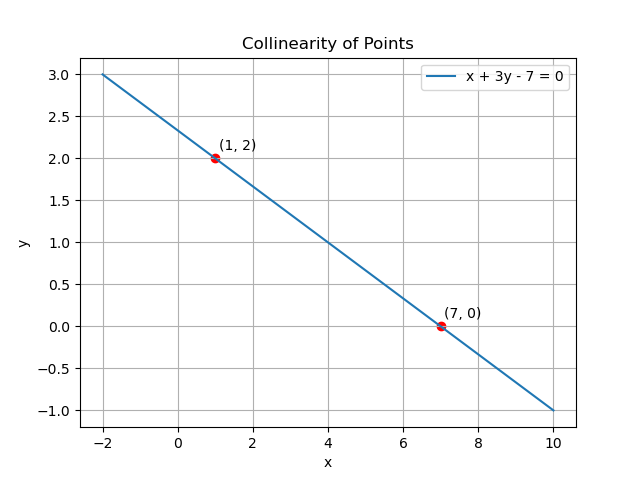
\includegraphics[width=0.7\columnwidth]{figs/fig1.png}
\caption{}
\label{fig:placeholder}
\end{figure}
\end{frame}
\section{C Code}
\begin{frame}[fragile]
\frametitle{C Code }
\begin{lstlisting}[language=C]
#include <stdio.h>

// Function to return relation value
int relation(int x, int y) {
    return x + 3*y - 7;
}

int main() {
    // Given points
    int x1 = 1, y1 = 2;
    int x2 = 7, y2 = 0;

    // Step 1: Compute slope
    float m = (float)(y2 - y1) / (x2 - x1);
  
\end{lstlisting}
\end{frame}
\begin{frame}[fragile]
 \begin{lstlisting}[language=C]
 printf("m=(y2-y1)/(x2-x1)=(%d-%d)/(%d-%d)=%.2f\n\n",
            y2, y1, x2, x1, m);
    // Step 2: Point-slope form
    printf("Step 2: Equation using point-slope form:\n");
    printf("(y-%d)=m(x-%d)\n\n", y1, x1);

    // Final Relation
    printf("Final Relation: x+3y-7=0\n");

    return 0;
}
    
\end{lstlisting}
\end{frame}

\section{Python Code}
\begin{frame}[fragile]
\frametitle{Python Code for Plotting}
\begin{lstlisting}[language=Python]
import numpy as np
import matplotlib.pyplot as plt

# Equation: x + 3y - 7 = 0 
y = (7 - x)/3
x_vals = np.linspace(-2, 10, 100)
y_vals = (7 - x_vals) / 3

plt.plot(x_vals, y_vals, label="x+3y-7=0")

# Given points
points = [(1,2), (7,0)]
for p in points:
    plt.scatter(p[0], p[1], color='red')
    plt.text(p[0]+0.1, p[1]+0.1, f"{p}")

plt.xlabel("x")
plt.ylabel("y")
\end{lstlisting}
\end{frame}
\begin{frame}[fragile]
\begin{lstlisting}[language=python]
plt.title("Collinearity of Points")
plt.legend()
plt.grid(True)
plt.savefig('../figs/fig1.png')
plt.show()

\end{lstlisting}
\end{frame}
\end{document}

